\section{Durchführung}
\label{sec:Durchführung}

Es wird ein Aufbau gemäß der in Abbildung \ref{fig:bild4} dargestellten Schaltskizze
verwendet.

\begin{figure} [H]
    \centering
    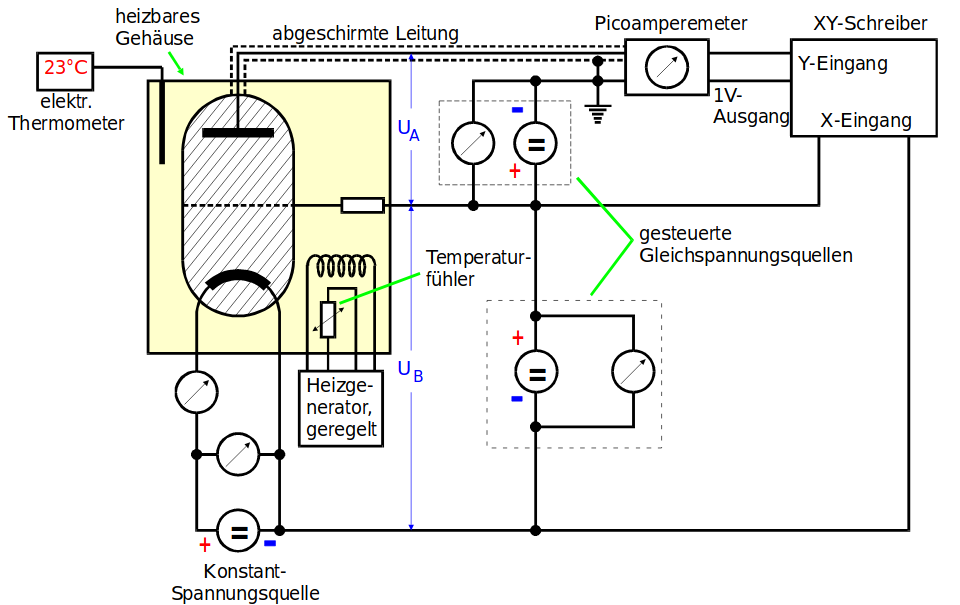
\includegraphics{content/bild4.png}
    \caption{Schaltplan des Franck-Hertz-Versuchs}
    \label{fig:bild4}
  \end{figure}

  Zusätzlich zu den zuvor beschriebenen Elektroden im Vakuumglas werden
  ein Heizgenerator, Temperaturfühler und ein XY-Schreiber zur Aufzeichnung der
  Franck-Hertz-Kurven verwendet. Außerdem lassen sich die Spannungen zeitpropotional
  innerhalb des Intervalls

  \begin{equation*}
      \SI{0}{\volt} \geq U_\text{B}, U_\text{A} \geq \SI{60}{\volt}
  \end{equation*}

  einstellen und der Auffängerstrom $I_\text{A}$ kann an einem Picoamperemeter abgelesen werden.

  Znächst wird die integrale Energieverteilung der beschleunigten Elektronen gemessen, indem
  $I_\text{A}$ in Abhängigkeit von $U_\text{A}$ und bei einer konstanten
  Bremsspannung $U_\text{B} = \SI{11}{\volt}$ aufgezeichnet wird.

  Dabei wird $U_\text{A}$ an den X-Eingang des XY-Schreibers geschlossen und dieser so geeicht,
  dass das gesamte Spannungsintervall aufgenommen werden kann. Diese Messung erfolgt einmal
  bei Raumtemperatur und ein weiteres Mal im Intervall 

\begin{equation*}
    \SI{140}{\degree\celsius} \geq T \geq \SI{160}{\degree\celsius} \; .
\end{equation*}

Danach werden drei Franck-Hertz-Kurven für $U_\text{A} =\SI{1}{\volt}$ und bei Temperaturen im Intervall

\begin{equation*}
    \SI{160}{\degree\celsius} \geq T \geq \SI{200}{\degree\celsius} \; .
\end{equation*}

für verschiedene $U_\text{B}$ gemessen.
Diesmal wird dazu $U_\text{B}$ an den X-Eingang des XY-Schreibers angeschlossen.

Zuletzt wird zur Bestimmung der Ionisationsenergie die Franck-Hertz-Kurve für $U_\text{A} = \SI{-30}{\volt}$
und im Temperaturintervall 

\begin{equation*}
    \SI{100}{\degree\celsius} \geq T \geq \SI{110}{\degree\celsius} \; .
\end{equation*}

gemessen.
